% ============================================================
%  sections/05d_pareto.tex
% ============================================================
\subsection{Pareto Frontier Analysis}
\label{sec:pareto}

Figure~\ref{fig:pareto_dashboard} shows the 6-panel performance
dashboard, and Figures~\ref{fig:pareto_size}--\ref{fig:pareto_lat}
show individual Pareto frontiers.

\begin{figure}[h]
  \centering
  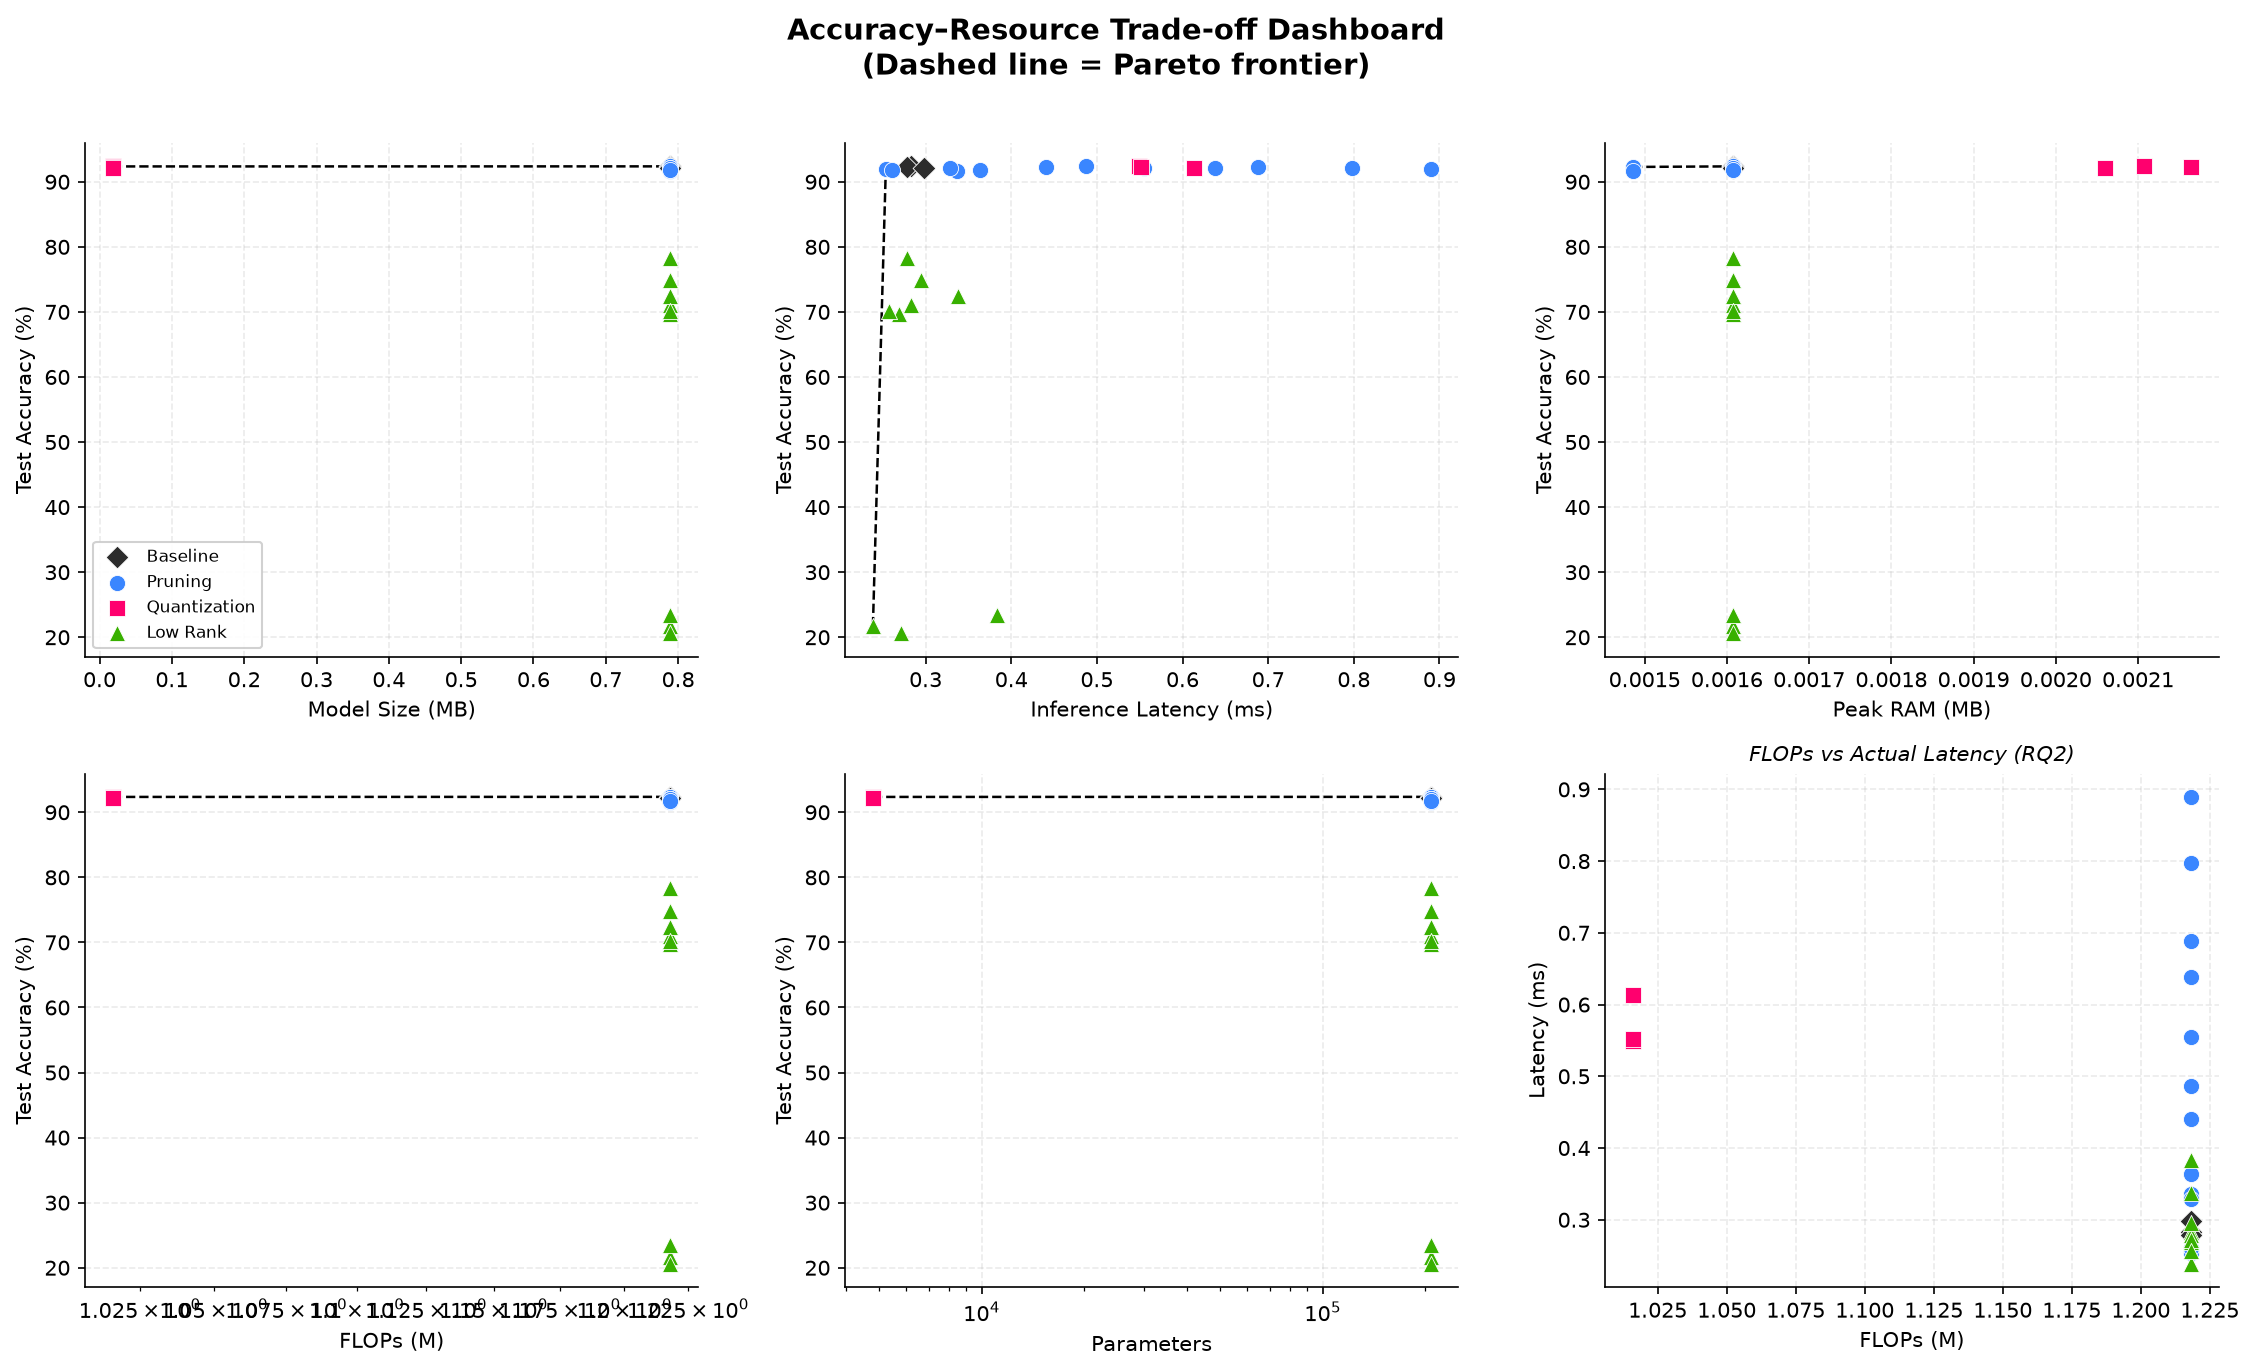
\includegraphics[width=\columnwidth]{figures/pareto_dashboard.png}
  \caption{6-panel performance dashboard.
  Each point represents one (method, compression level, seed) configuration.
  Stars indicate Pareto-optimal points. Baseline (FP32, uncompressed)
  shown as dashed reference.}
  \label{fig:pareto_dashboard}
\end{figure}

\begin{figure}[h]
  \centering
  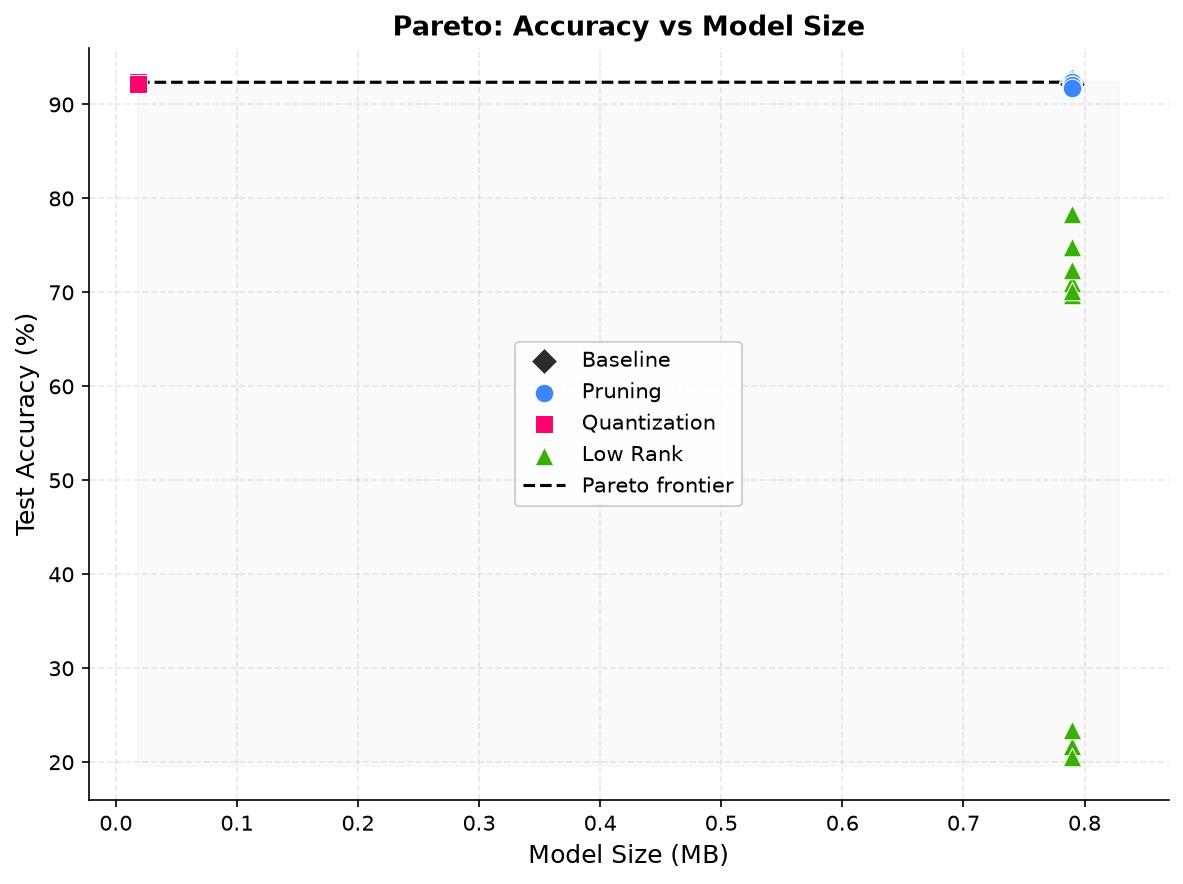
\includegraphics[width=0.9\columnwidth]{figures/pareto_accuracy_vs_size.png}
  \caption{Pareto frontier: test accuracy vs.\ model size.
  Dynamic INT8 quantization dominates: it achieves the best
  accuracy--size trade-off by 4$\times$ model size reduction.}
  \label{fig:pareto_size}
\end{figure}

\begin{figure}[h]
  \centering
  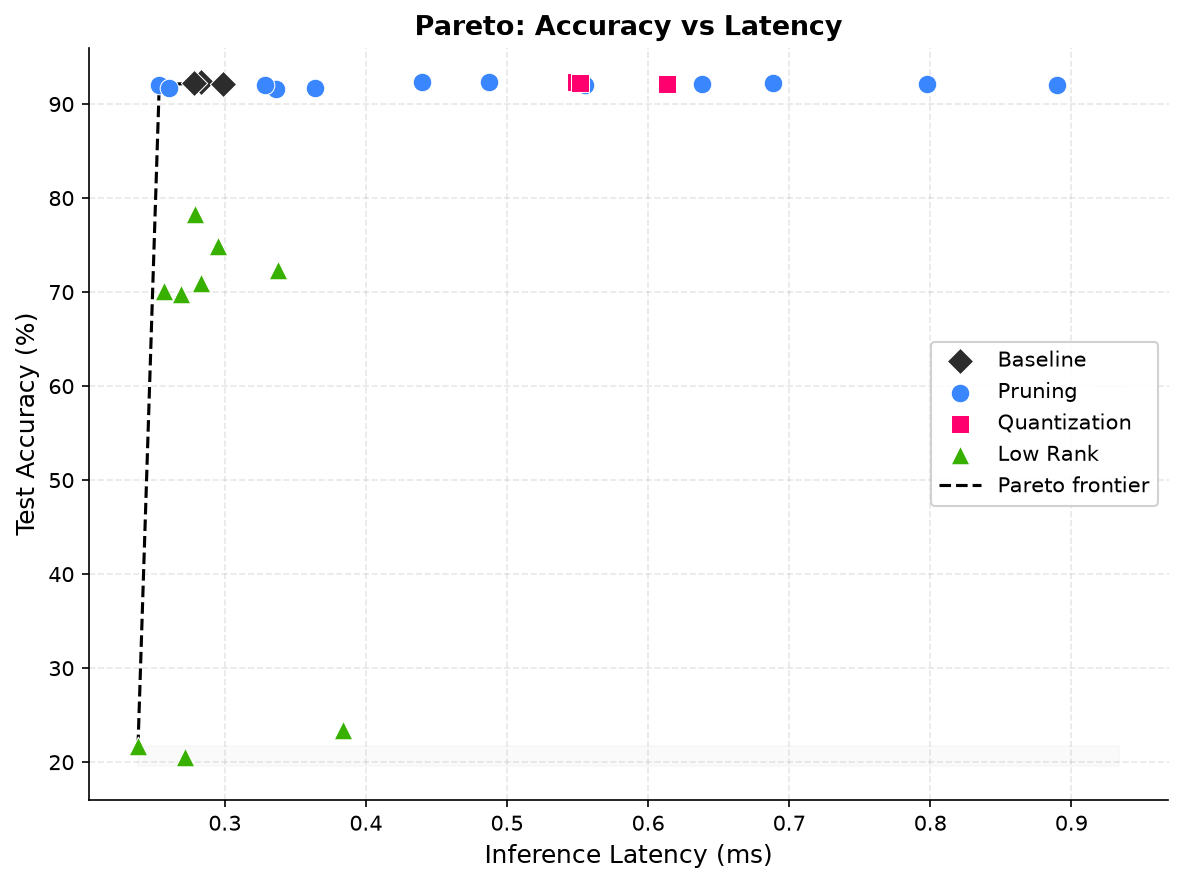
\includegraphics[width=0.9\columnwidth]{figures/pareto_accuracy_vs_latency.png}
  \caption{Pareto frontier: test accuracy vs.\ inference latency.
  Unstructured pruning does \emph{not} improve latency despite
  reducing theoretical FLOPs.
  Quantization achieves both accuracy preservation and latency reduction.}
  \label{fig:pareto_lat}
\end{figure}

\paragraph{RQ3 answer.}
Across all three Pareto dimensions (accuracy--size, accuracy--latency,
accuracy--RAM), \textbf{dynamic INT8 quantization dominates}:
it is the only method that simultaneously reduces size \emph{and}
latency while preserving accuracy.
Pruning achieves Pareto improvements on the accuracy--FLOPs frontier
(not shown) but not on the accuracy--latency frontier, due to the
hardware gap discussed in Section~\ref{sec:pruning_results}.
